\newpage
\section{Introdução}

O strain gage possui grande utilidade no ramo da Engenharia. Trata-se de um sensor elétrico cujo principio de funcionamento é baseado na variação da resistência quando submetido a uma deformação.

Consta essencialmente de uma grade metálica sensível, ligada a uma base que se cola à peça ou estrutura que se deseja monitorar. O fio sensível tem, na maioria dos extensômetros, um diâmetro aproximado de 0,01mm e é constituído por ligas metálicas especiais. A grade fica embebida entre duas folhas de papel ou dentro de uma fina película de plástico. Nas extremidades do fio sensível estão soldados dois outros de maior diâmetro que constituem o elemento de ligação do extensômetro ao circuito de medição.

Existem dois tipos básicos de strain gages:

\begin{itemize}
    \item \textbf{Wire gage}: extensômetro de fio;
    \item \textbf{Foil gage}: extensômetro de película.
\end{itemize}

As primeiras aplicações da extensometria ocorreram por volta de 1856 quando Thomsom (Lord Kelvin) realizou experimentos com ferro e cobre e concluiu que a resistência elétrica de ambos mudava quando estes sofriam deformações. Para tal procedimento, ele utilizou a chamada "Ponte de Wheatstone" e um galvanômetro (indicador). 

\begin{figure}[H]
    \centering
    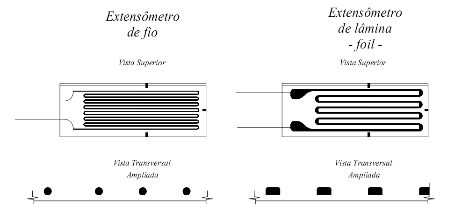
\includegraphics[scale=0.9]{img/fi1.png}
    \caption{\textit{Strain gauge}.}
    \label{f_fi1}
\end{figure}

Porém foi só a partir do século passado que o strain gage passou a ser considerado o único sistema de medição de deformação que contempla todas as propriedades requeridas para o desempenho ótimo, capaz de fornecer medidas com precisão de 10-6 mm/mm.

Como sabemos, um extensômetro elétrico transforma uma deformação, numa variação proporcional da sua resistência elétrica, de forma que a relação entre a deformação aplicada ($\epsilon = \frac{\Delta L}{L_0}$) e tal variação de resistência é dada por: 

\[ 
    \frac{\Delta R}{R_0} = k \epsilon.
\]

Onde $R_0$ é a resistência inicial do extensômetro, $\Delta R$ é a variação dessa resistência devido à deformação e $k$ é o chamado fator do extensômetro, um valor
característico de cada tipo e calculado experimentalmente.

A ponte de Wheatstone está representada na Figura \ref{f_fi2}:

\begin{figure}[H]
    \centering
    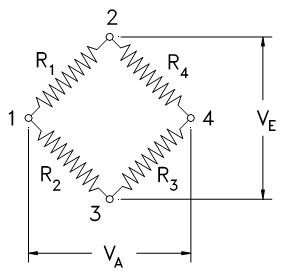
\includegraphics[scale=0.5]{img/fi2.png}
    \caption{Ponte de Wheatstone.}
    \label{f_fi2}
\end{figure}

O circuito da ponte contém quatro resistências, $R_1$ a $R_4$. Se os nós 2 e 3 forem ligados a uma fonte de potência com voltagem conhecida $V_E$, aparecerá uma outra diferença de potencial $V_A$, entre os nós 1 e 4. O valor de $V_A$ depende dos quocientes entre resistências $\frac{R_1}{R_2}$ e $\frac{R_3}{R_4}$. Tem-se então a seguinte equação: 

\[
\frac{V_A}{V_E} = \frac{R_1}{R_1 + R_2} - \frac{R_4}{R_3 + R_4}.
\]

A ponte de Wheatstone está em equilíbrio quando:

\[
\frac{V_A}{V_E} = 0.
\]

Assim é necessário que se verifique:

\[ R_1 = R_2 = R_3 = R_4 \]

ou  

\[ \frac{R_1}{R_2} = \frac{R_3}{R_4} \].

Partindo então do princípio que uma dada ponte de Wheatstone está equilibrada, qualquer variação de resistência em uma ou mais resistências da ponte, provocará uma diferença de potencial $V_A$ diferente de zero. 

Sabe-se também que a resistência elétrica está relacionada com o comprimento e área transversal de um dado material da seguinte forma:

\[ 
    R = \rho \frac{L}{A}.
\]

A partir daí é fácil concluir que quando uma barra metálica sofre uma variação do seu comprimento, por tração ou compressão, também acarreta uma variação do seu volume, resultando a diminuição (no caso da tração) ou um aumento (no caso da compressão) da área da seção transversal desta barra, e consequentemente variando sua resistência. 

A ponte de Wheatstone converte essa variação de resistência em uma tensão na saída, da ordem de mV ou V; esses dados de variação podem ser coletados por diferentes voltímetros e até mesmo ser processado num microcomputador para um melhor monitoramento do objeto analisado.